{{TABLE:frontier}}
\begin{figure}[H]
\centering
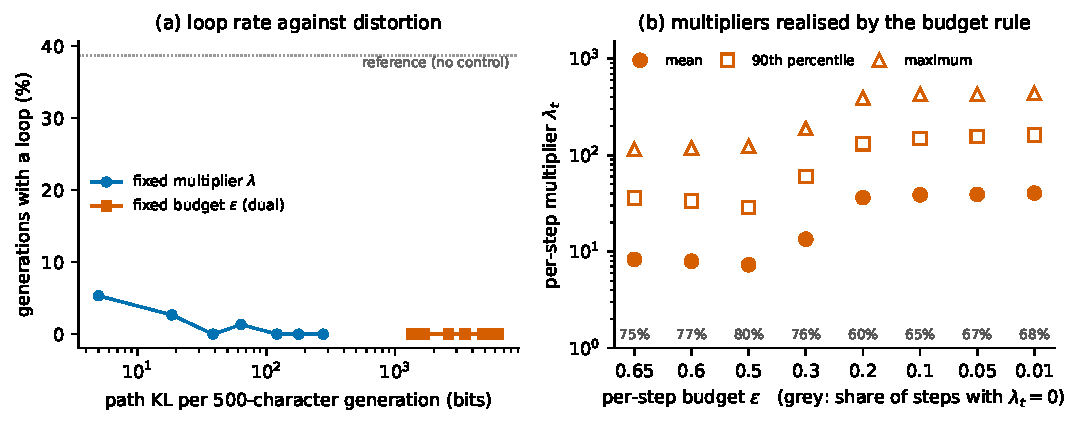
\includegraphics[width=\textwidth]{figures/fig_frontier.pdf}
\caption{Primary model, $T=0.10$, 75 generations per setting. (a) Share of generations with a detected loop against the path KL per 500-character generation, for the fixed-price rule (one $\lambda$ for the whole generation) and the fixed-budget rule (one $\varepsilon$ re-solved at every step); the budget $\varepsilon=1$ (no active constraint) coincides with the reference and has zero KL. (b) Per-step multipliers $\lambda_t$ that the budget rule realizes for $\varepsilon<1$: mean, 90th percentile and maximum over steps, and the share of steps at which the constraint is inactive ($\lambda_t=0$).}\label{fig:frontier}
\end{figure}
Table~\ref{tab:frontier} and Figure~\ref{fig:frontier} give the sweep (75 generations per setting, seeds 1--5 of the 15 prompts; the reference loops in 29 of them). The control behaves as it should: the budget $\varepsilon=1$ reproduces the reference generation by generation (75 of 75 generations have the same loop onset, total KL $\le6\cdot10^{-6}$ bits). The two families then differ sharply. The fixed price moves smoothly with $\lambda$: 15/75 loops at 0.3 bits ($\lambda=0.25$), 9/75 at 1.2 bits, 4/75 at 5.0 bits, 2/75 at 18.5 bits (4/150 in the full run of Table~\ref{tab:primary}) and 0/75 at 38.6 bits ($\lambda=3$). The budget rule has no setting with an intermediate count on this grid: the count drops from 29/75 at $\varepsilon=1$ to 0/75 at $\varepsilon=0.95$, at 458 bits, and stays at 0/75 for every tighter budget, at 458 to 6364 bits (cost rising as the budget tightens). Among settings with zero observed loops the cheapest budget costs 12 times the cheapest fixed price ($\lambda=3$; prompt-bootstrap 95\% interval 11--12) and 25 times the fixed price with 2/75 loops; the tightest costs 165 times ($\lambda=3$, interval 156--174) and 23 times the strongest fixed price tested ($\lambda=12$, 277 bits). This is a comparison of cost at similar \emph{observed} counts. A count of 0/75 has a 95\% upper limit of 4.8\% on the true rate, so it does not show that two settings have equal loop probabilities; for that, the count of the budget rule would have to be resolved between $\varepsilon=0.95$ and 1, a range of the grid that was not subdivided further.

The multipliers explain the cost, as in Section~\ref{sec:small}. Wherever the budget rule is active ($\varepsilon<1$), the constraint is inactive ($\lambda_t=0$) at 60--80\% of steps, and where it acts it uses large multipliers: a 90th percentile of 26--163 and a maximum of 94--437 (mean over generations, Figure~\ref{fig:frontier}b), against a single $\lambda$ of 0.25--12 for the fixed-price rules. The price of risk it pays varies by two orders of magnitude within a generation, which is the dispersion that Proposition~\ref{prop:waste} identifies with excess cost. Two limits apply. The recurrence risk is a proxy and not the hazard, so the quantitative law is not tested here; and the average reference risk of about 0.69 is not the point at which the constraint becomes inactive, which is why the sweep extends to $\varepsilon=1$.
